\section{Introduction}

\label{sec:intro}

\begin{frame}{Visual Based Localization}
	Visual Based Localization (\textbf{VBL}) aims to recover the pose or position of a visual input query according to a known visual reference.
	\vfill	
	\begin{minipage}{0.4\linewidth}
	   \centering
		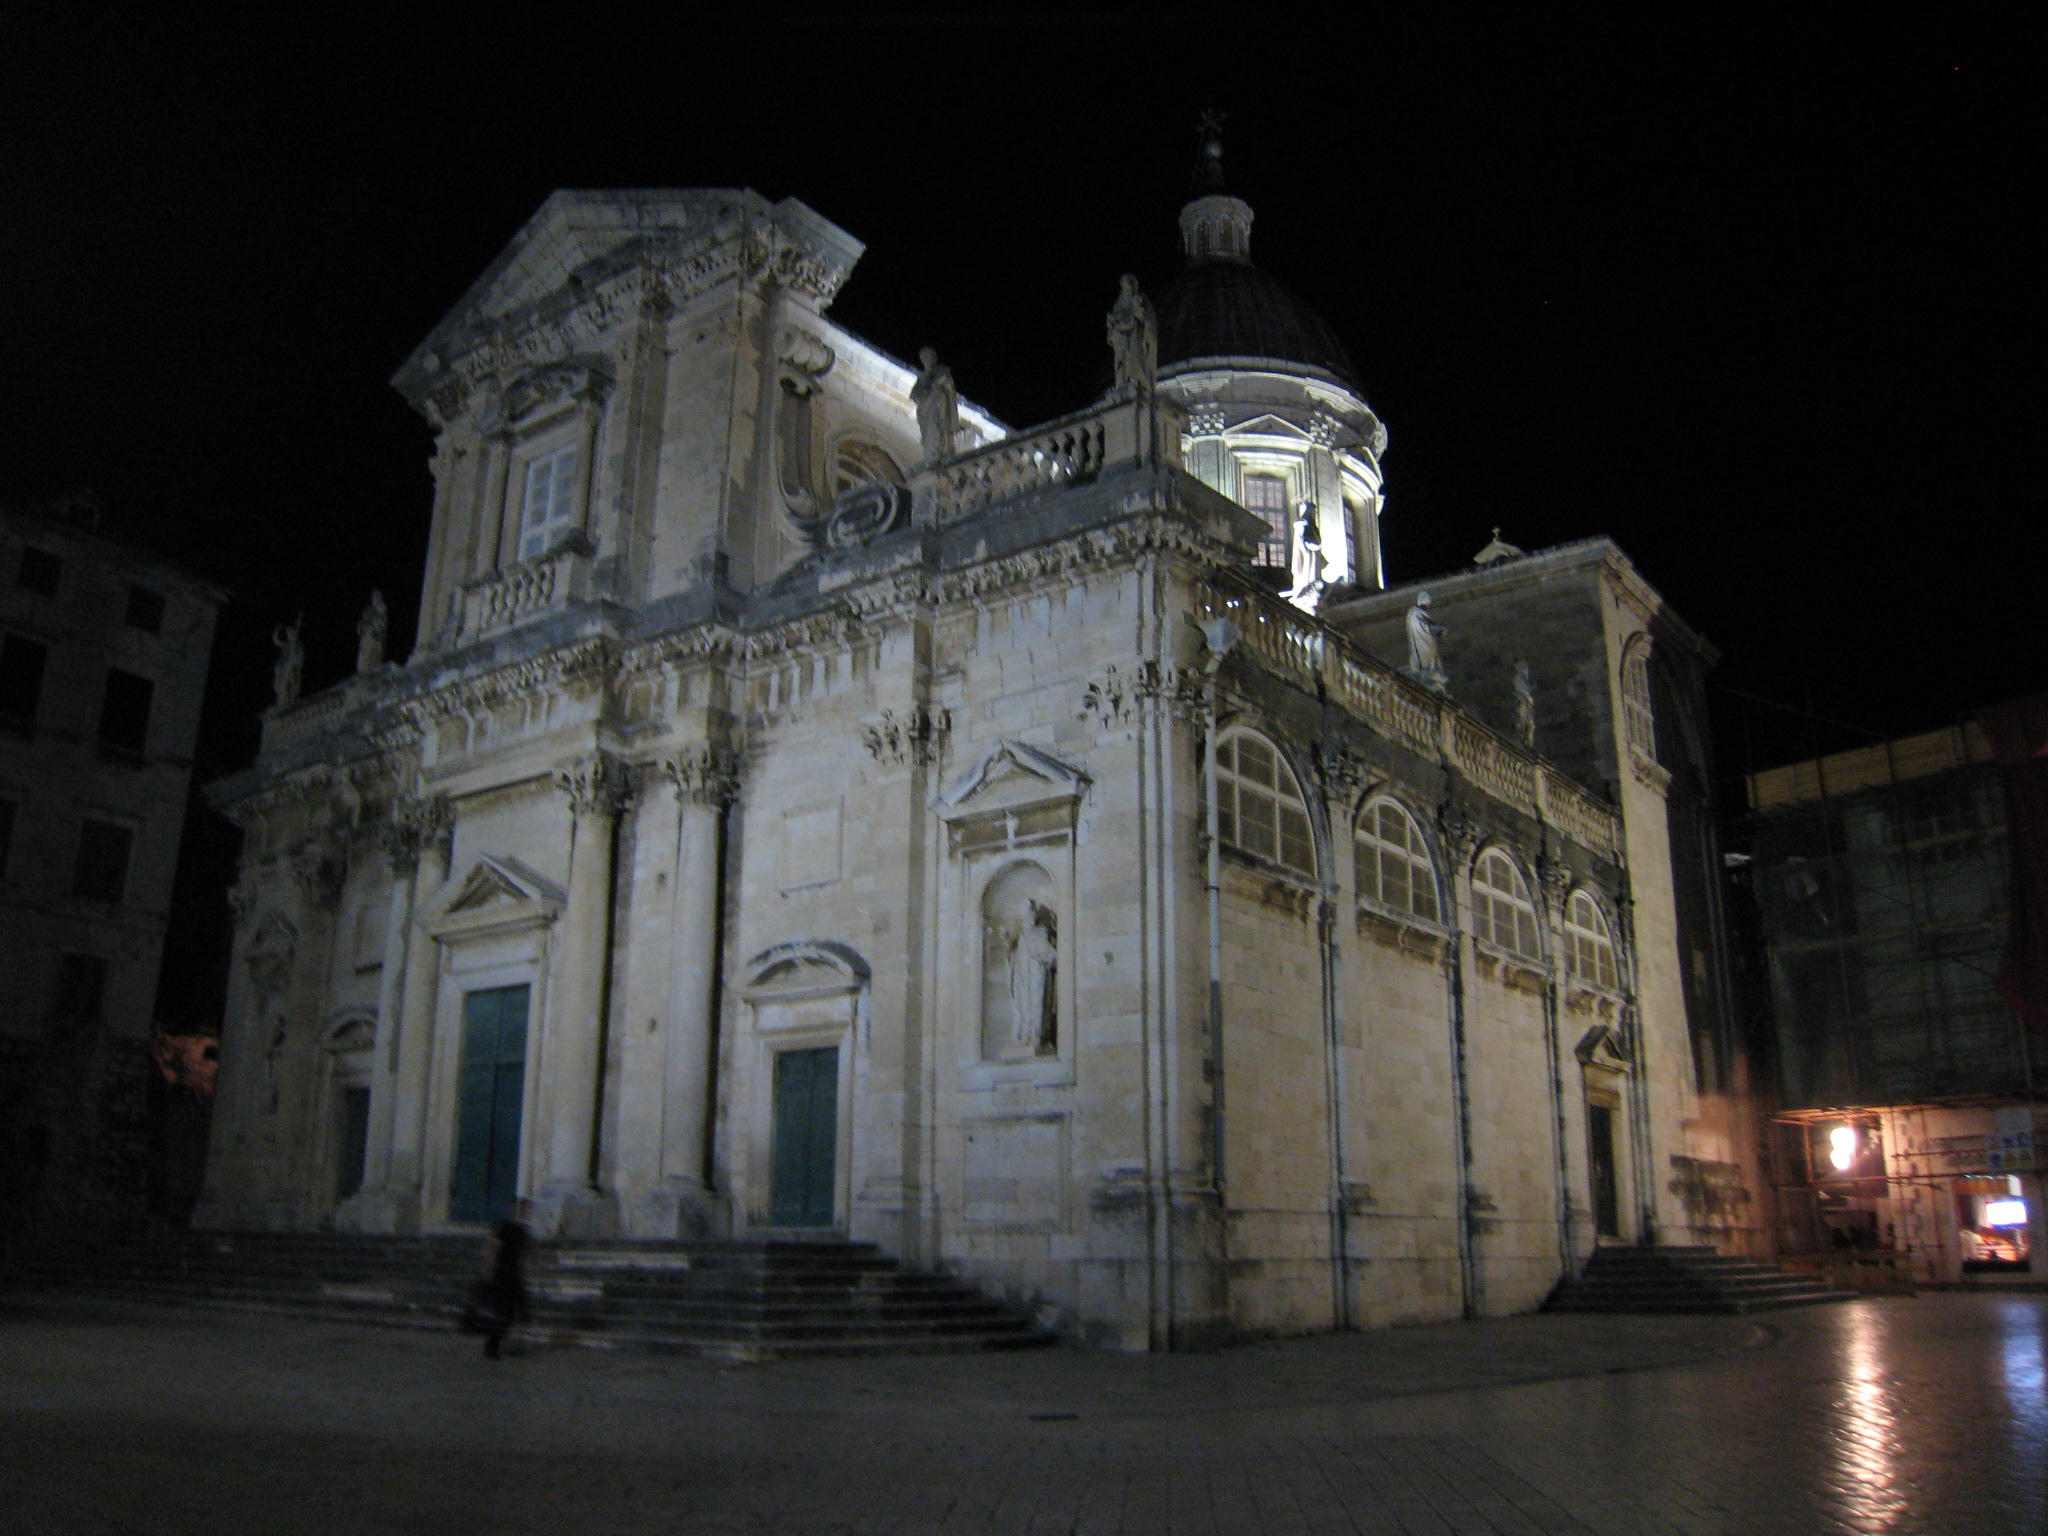
\includegraphics[width=\linewidth]{images/intro_fig/dubrovnik_night_query.jpg}
	\end{minipage}
	$\rightarrow$ \textbf{?} $\rightarrow$
	\begin{minipage}{0.4\linewidth}
	   \centering
		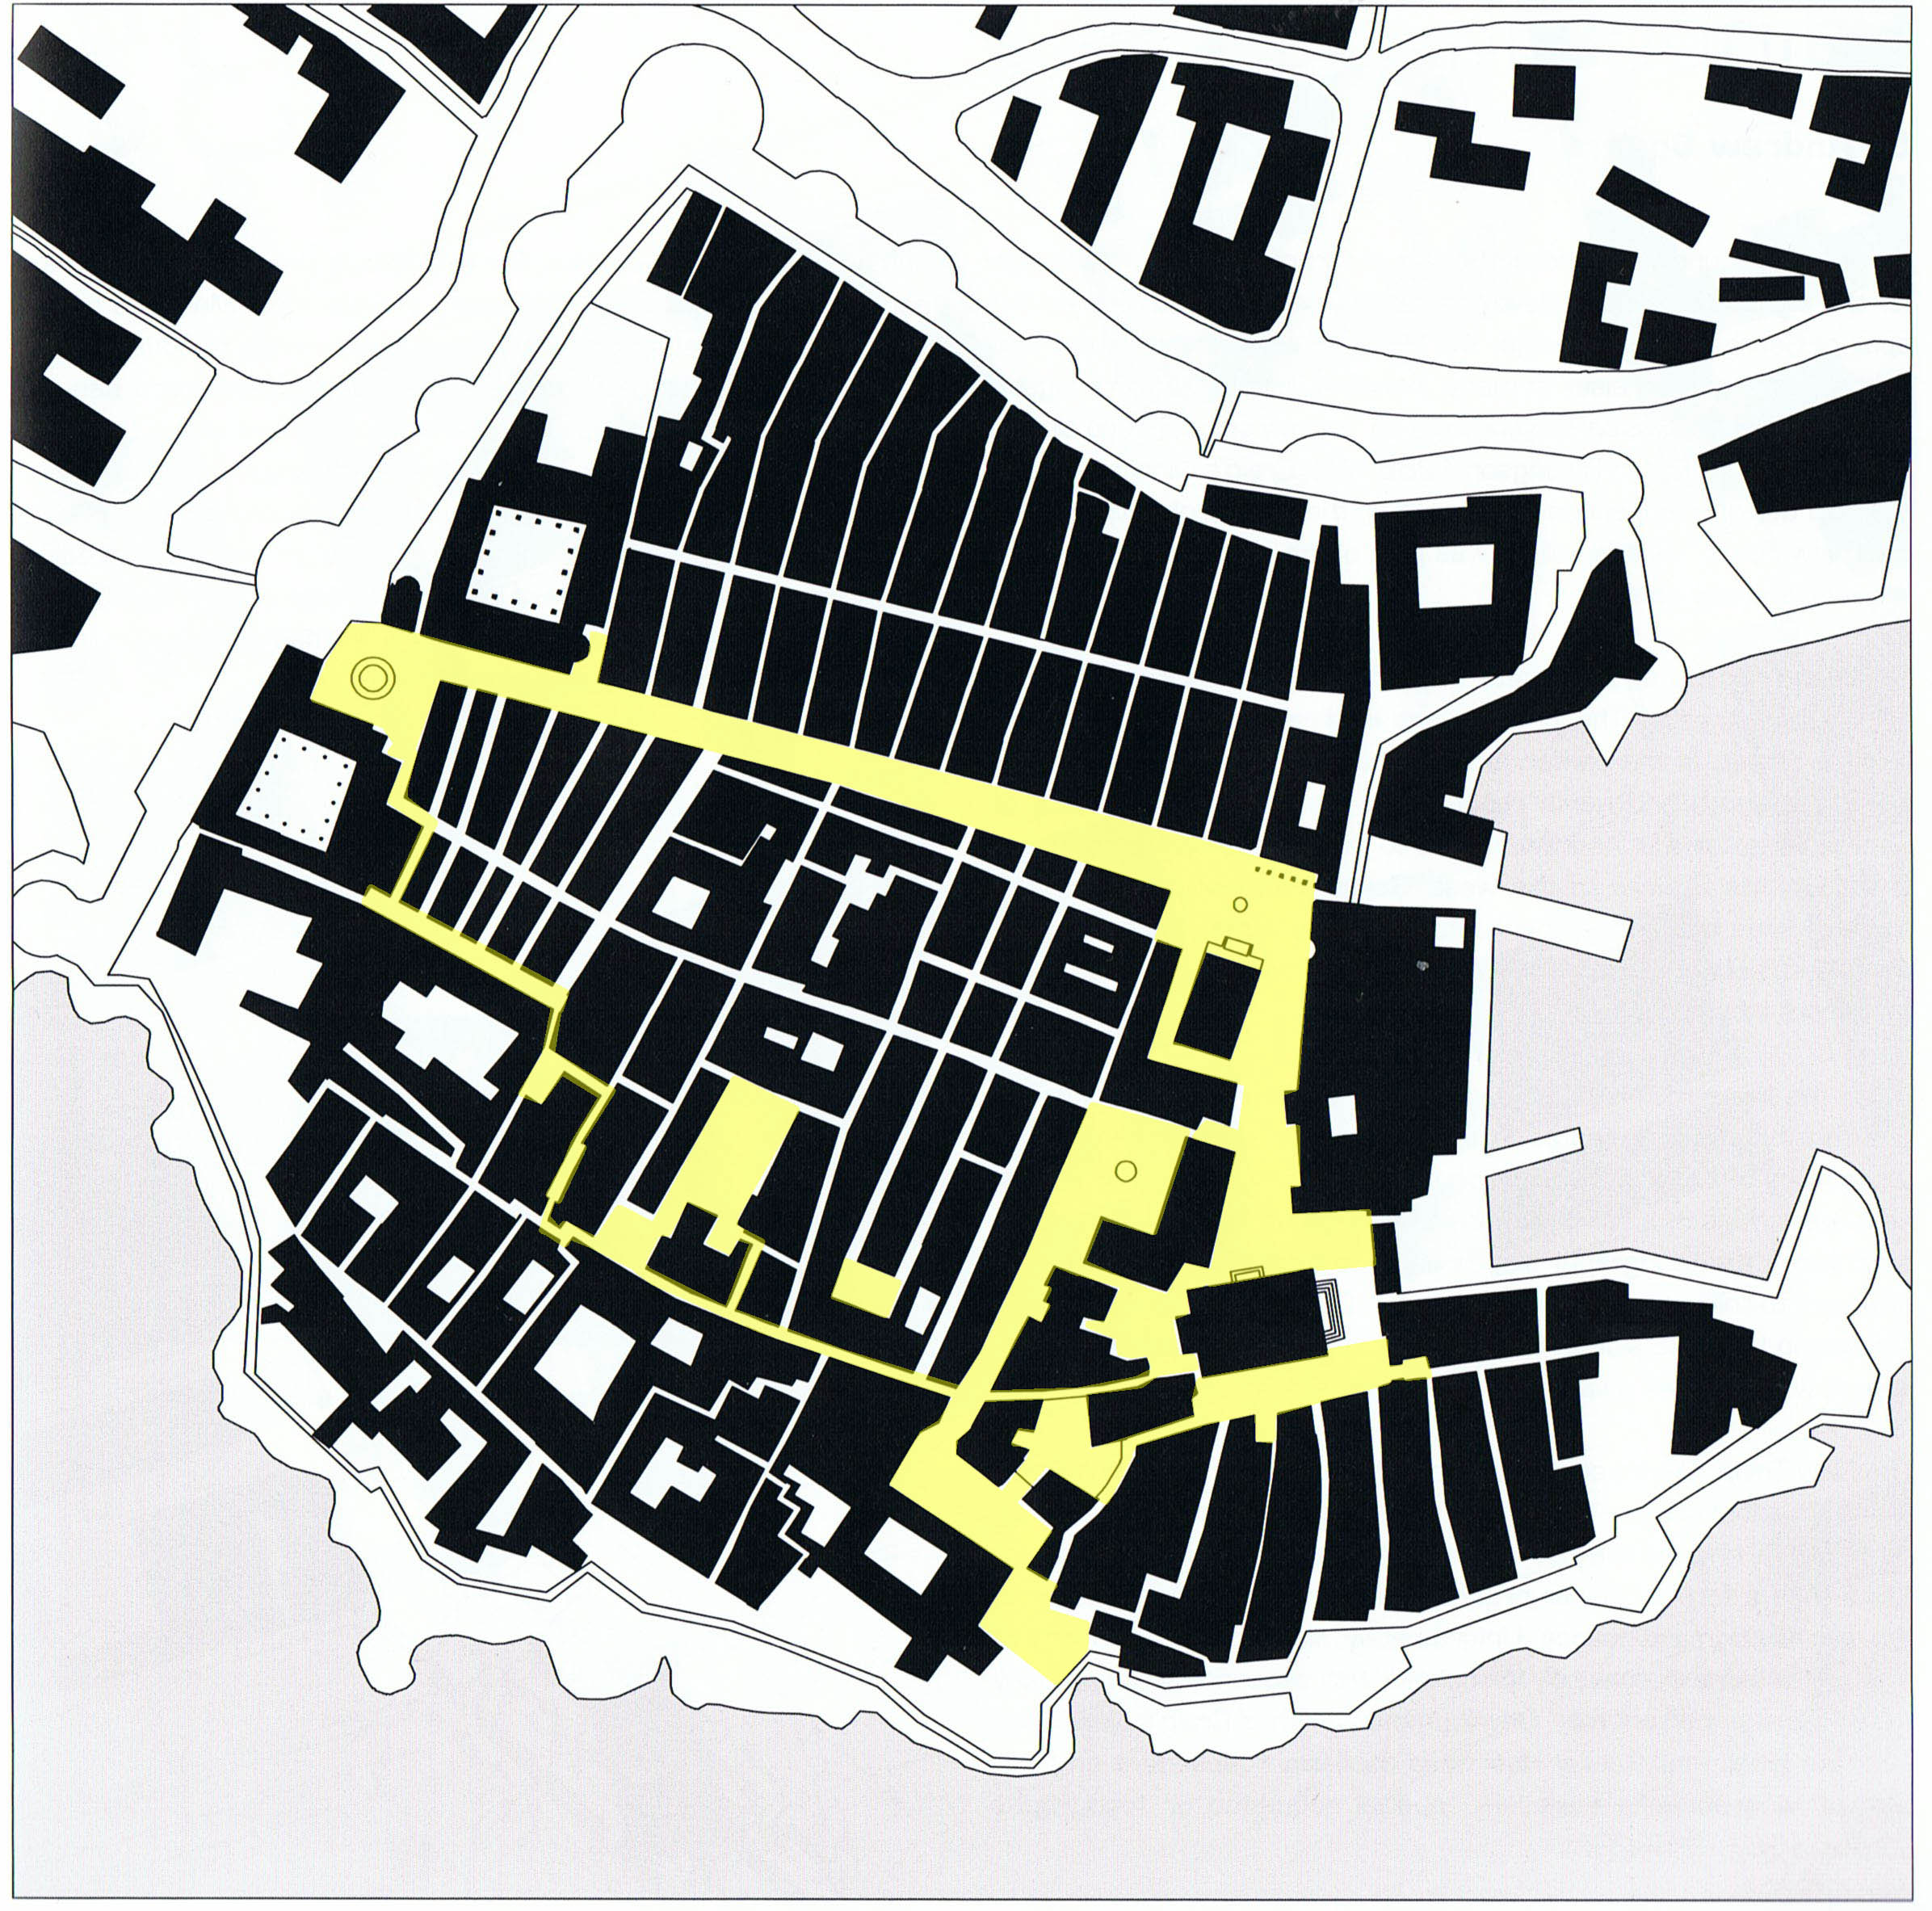
\includegraphics[width=\linewidth]{images/intro_fig/dubrovnik_map.jpg}
	\end{minipage}	
\end{frame}

\begin{frame}{Direct vs Indirect methods}
	Visual Based Localization (\textbf{VBL}) methods can be devided in two main categories~\cite{Piasco2017}:
	\vfill
	\begin{minipage}[t]{0.48\linewidth}
		\begin{block}{Direct methods}
			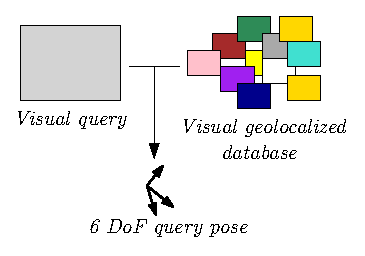
\includegraphics[width=0.9\textwidth]{vect/direct.eps}
			\begin{itemize}
				\item Accurate
				\item Position + orientation
				\item Small area
			\end{itemize}
		\end{block}
	\end{minipage}
	\hfill
	\uncover<2>{
	\begin{minipage}[t]{0.48\linewidth}
		\begin{block}{Indirect methods}
			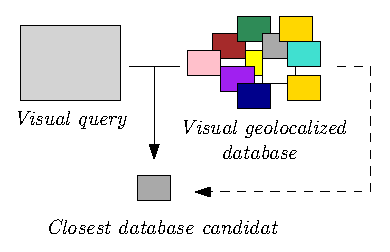
\includegraphics[width=0.9\textwidth]{vect/indirect.eps}		
			\begin{itemize}
				\item Coarse position
				\item Cover large area
				\item Fast
			\end{itemize}			
		\end{block}
	\end{minipage}	
	}
\end{frame}

\begin{frame}{Visual Based Localization: Indirect methods}
	VBL can be solved by retrieving the closest geo-referenced candidate in the database.
	\vfill
	\only<1>{
		\begin{minipage}{0.2\linewidth}
		   \centering
			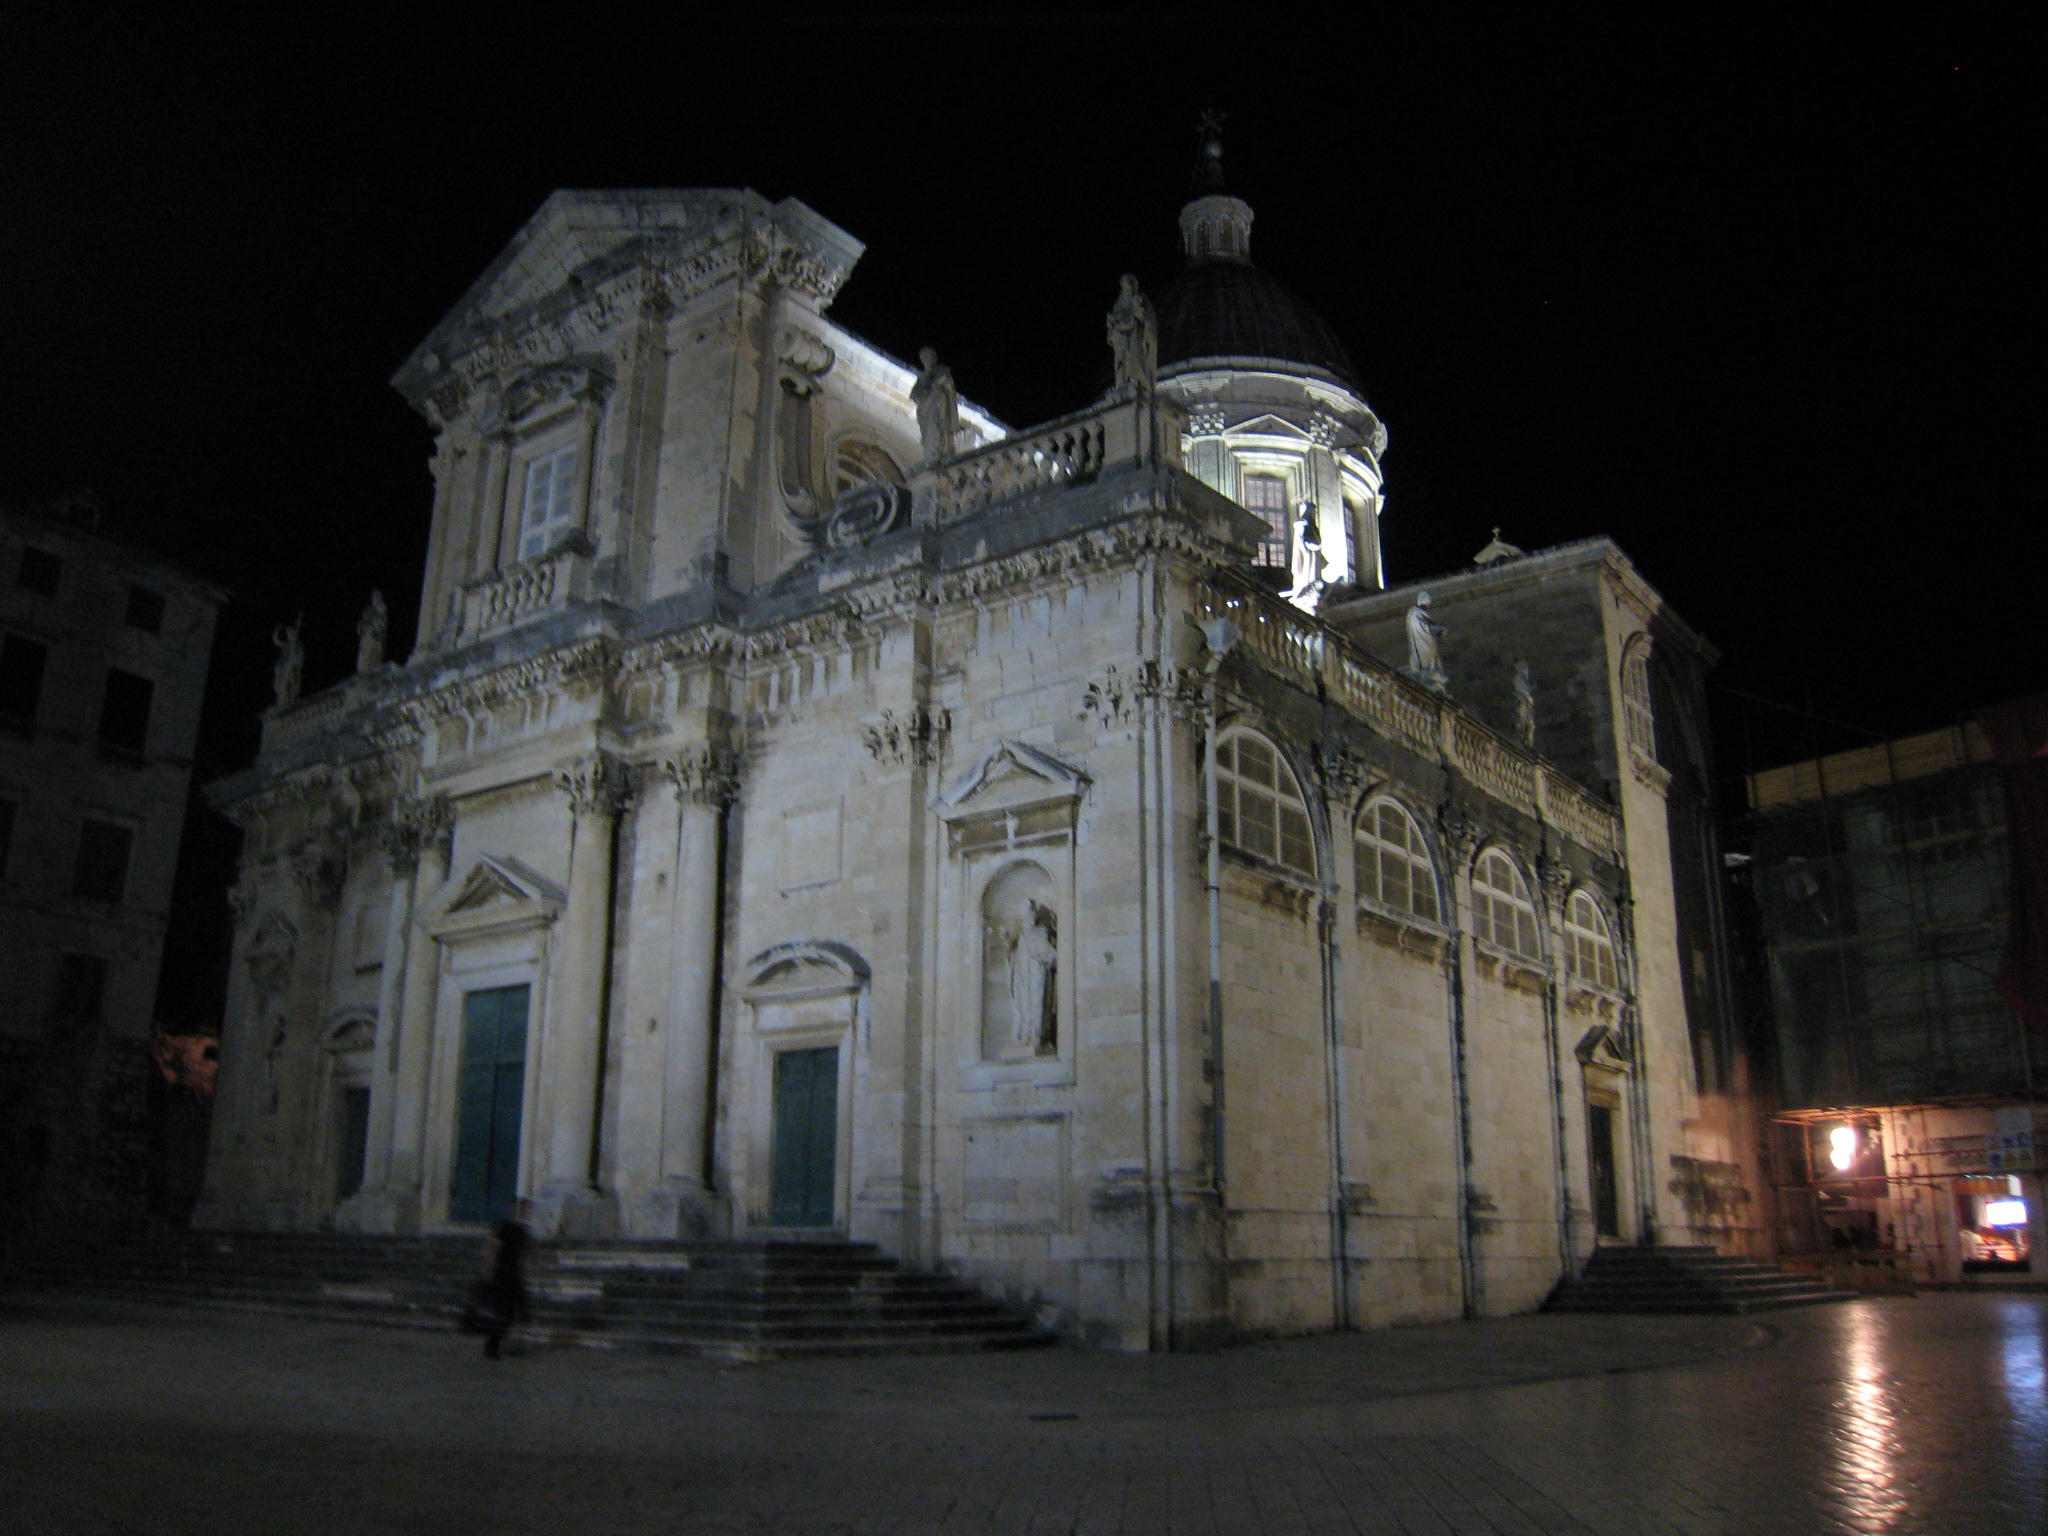
\includegraphics[width=\linewidth]{images/intro_fig/dubrovnik_night_query.jpg}
		\end{minipage}
		$\rightarrow$
		\begin{minipage}{0.75\linewidth}
		   \centering
			\begin{tabular}{c c c c}
				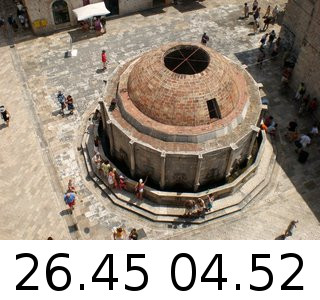
\includegraphics[width=0.18\textwidth]{images/intro_fig/dataset/1.jpg} & 
				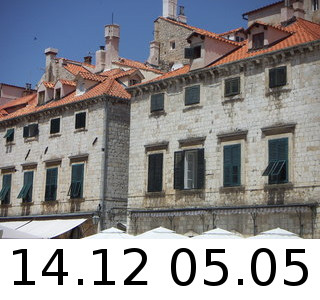
\includegraphics[width=0.18\textwidth]{images/intro_fig/dataset/2.jpg} & 
				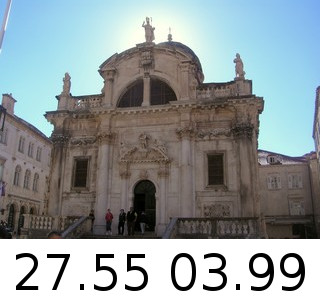
\includegraphics[width=0.18\textwidth]{images/intro_fig/dataset/3.jpg} & 
				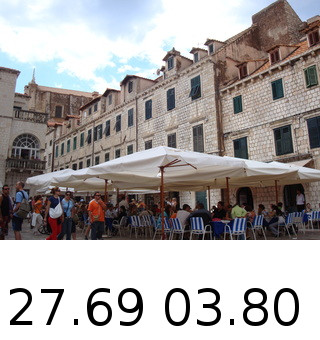
\includegraphics[width=0.18\textwidth]{images/intro_fig/dataset/5.jpg} \\
				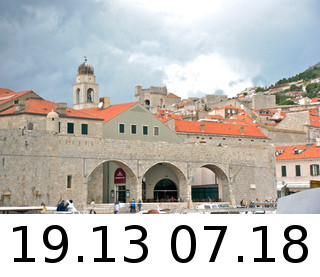
\includegraphics[width=0.18\textwidth]{images/intro_fig/dataset/6.jpg} &
				\multicolumn{3}{c}{	
					\multirow{3}{*}{
						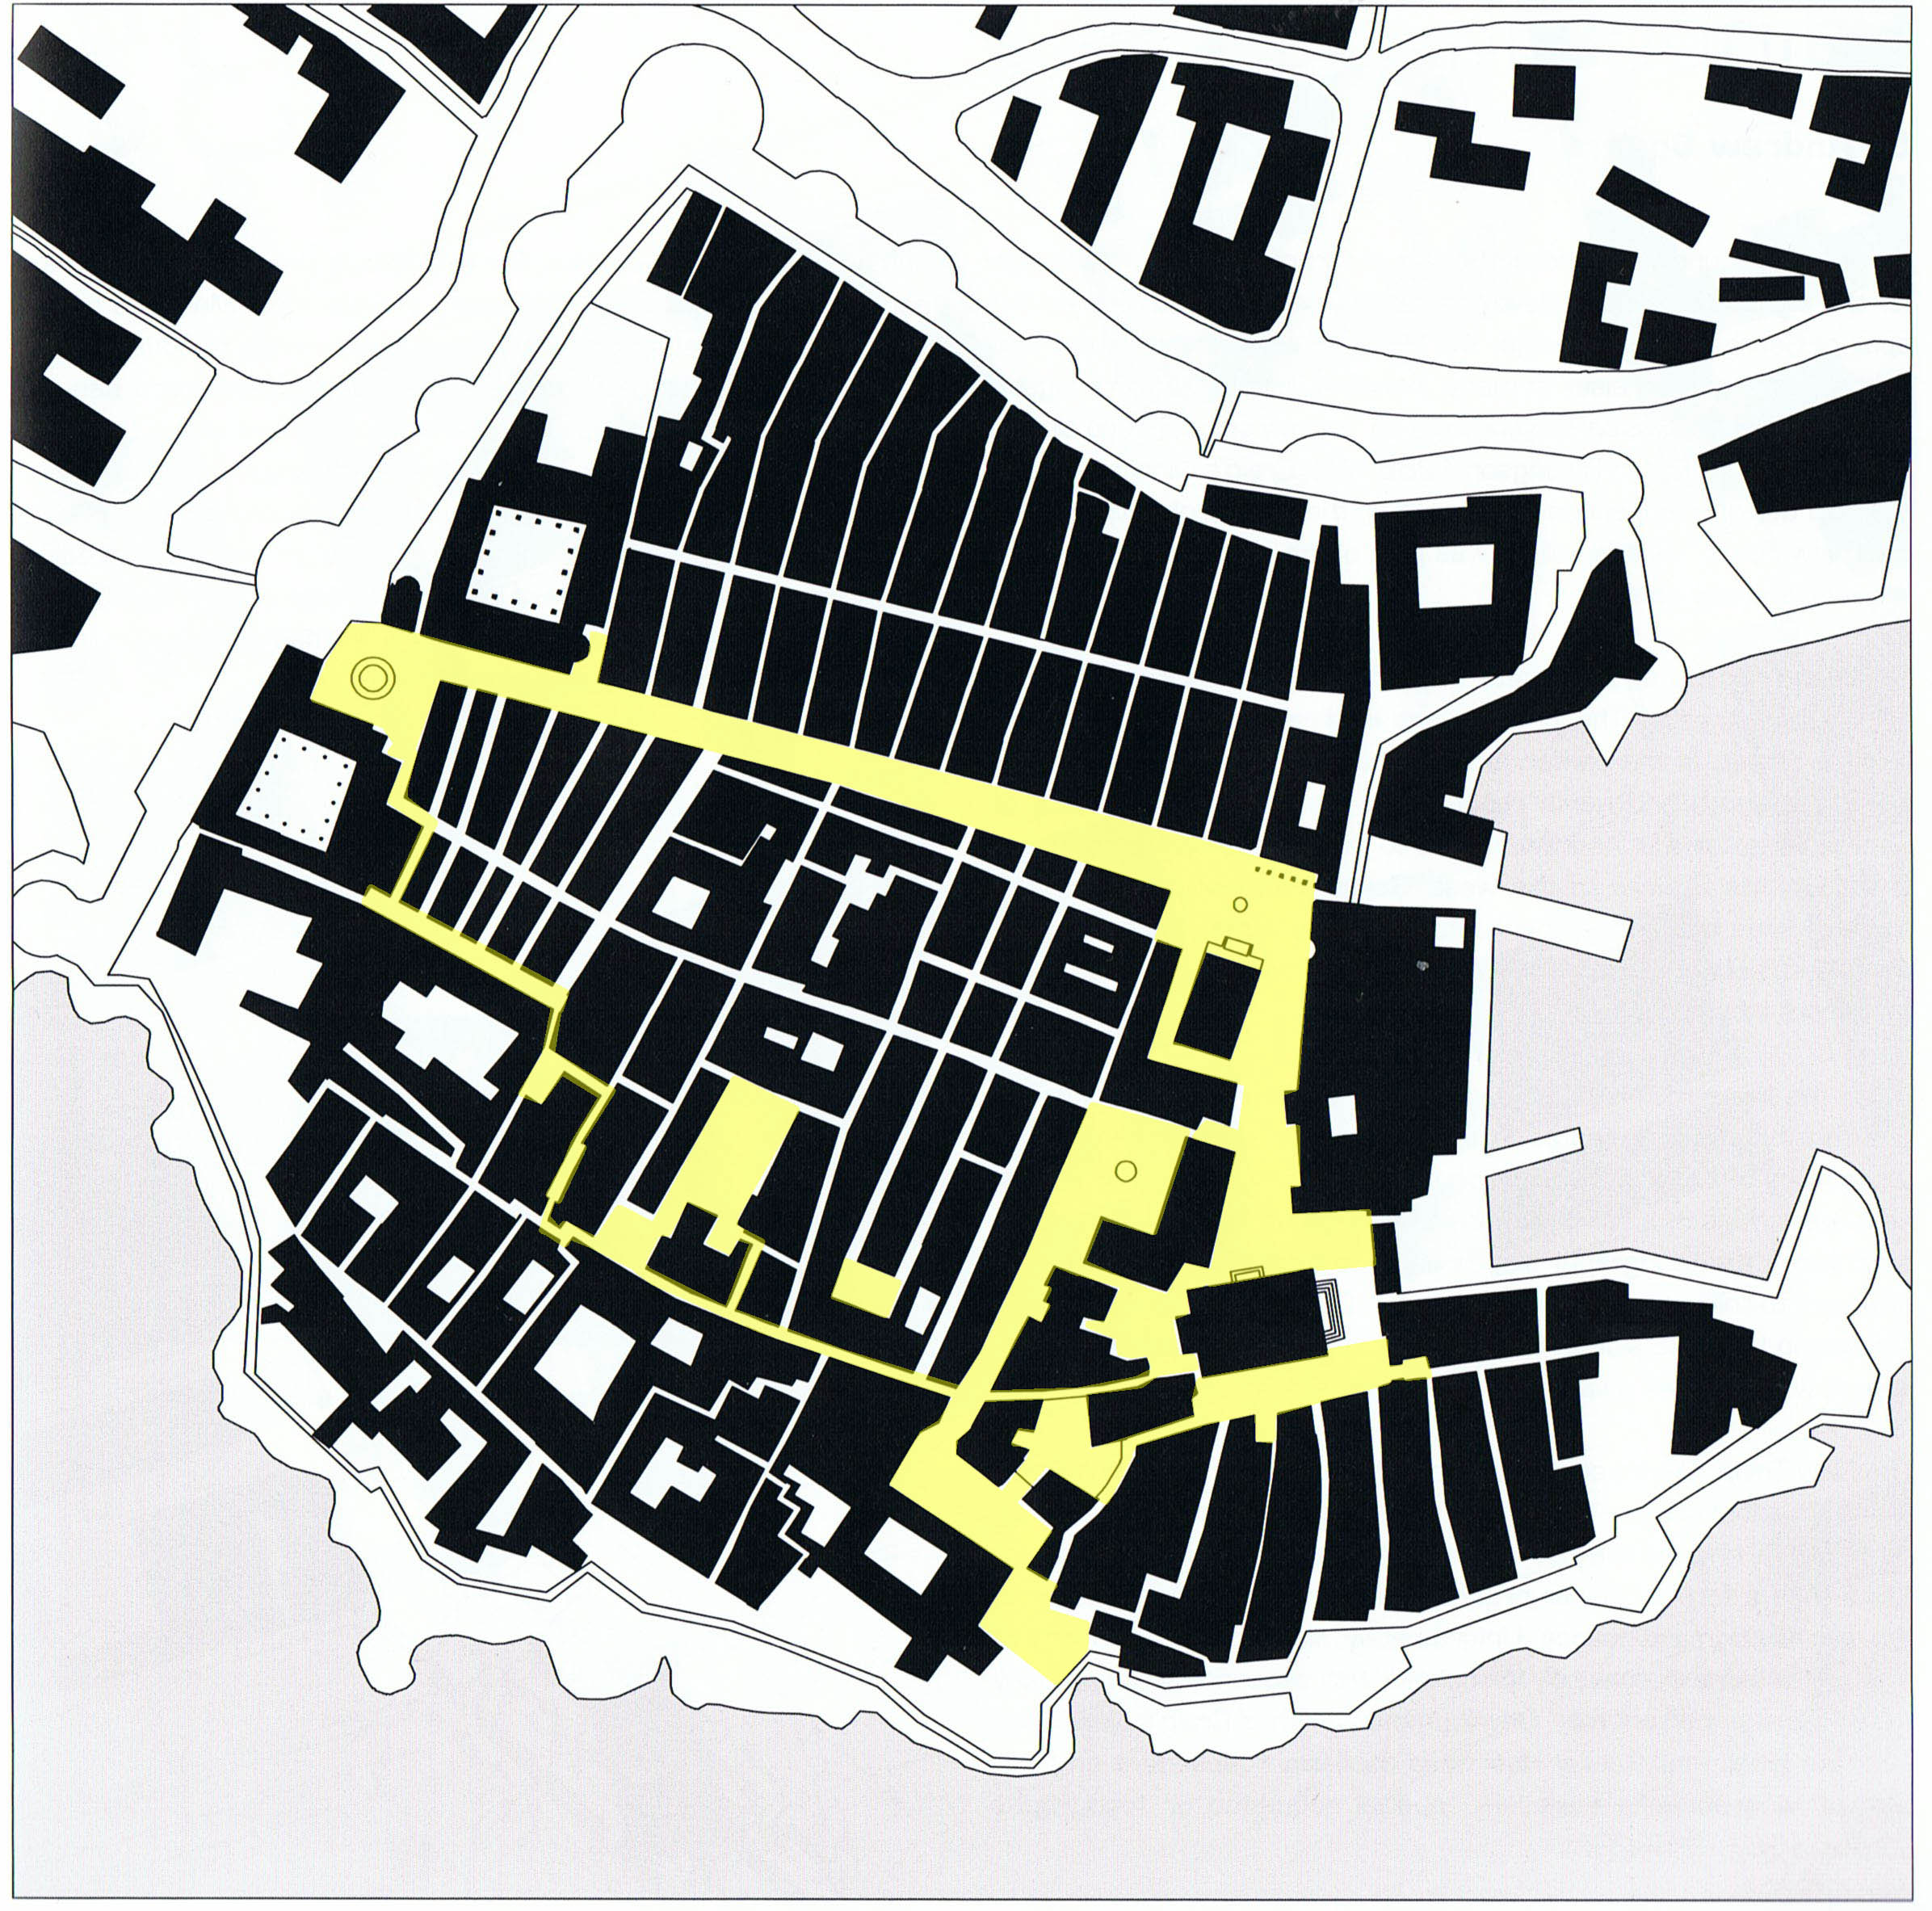
\includegraphics[width=0.40\textwidth]{images/intro_fig/dubrovnik_map.jpg}
					}
				} \\
				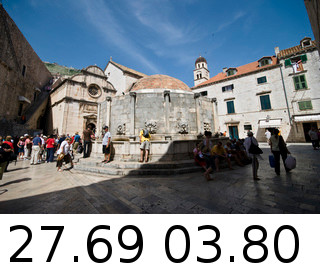
\includegraphics[width=0.18\textwidth]{images/intro_fig/dataset/7.jpg} \\
				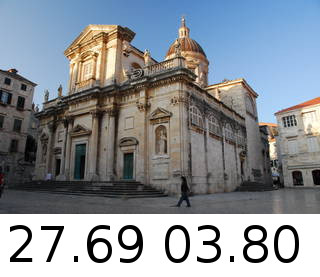
\includegraphics[width=0.18\textwidth]{images/intro_fig/dataset/8.jpg} \\
			\end{tabular}
		\end{minipage}
	}
	\only<2>{
		\centering
		\begin{minipage}{0.3\linewidth}
			\centering		
			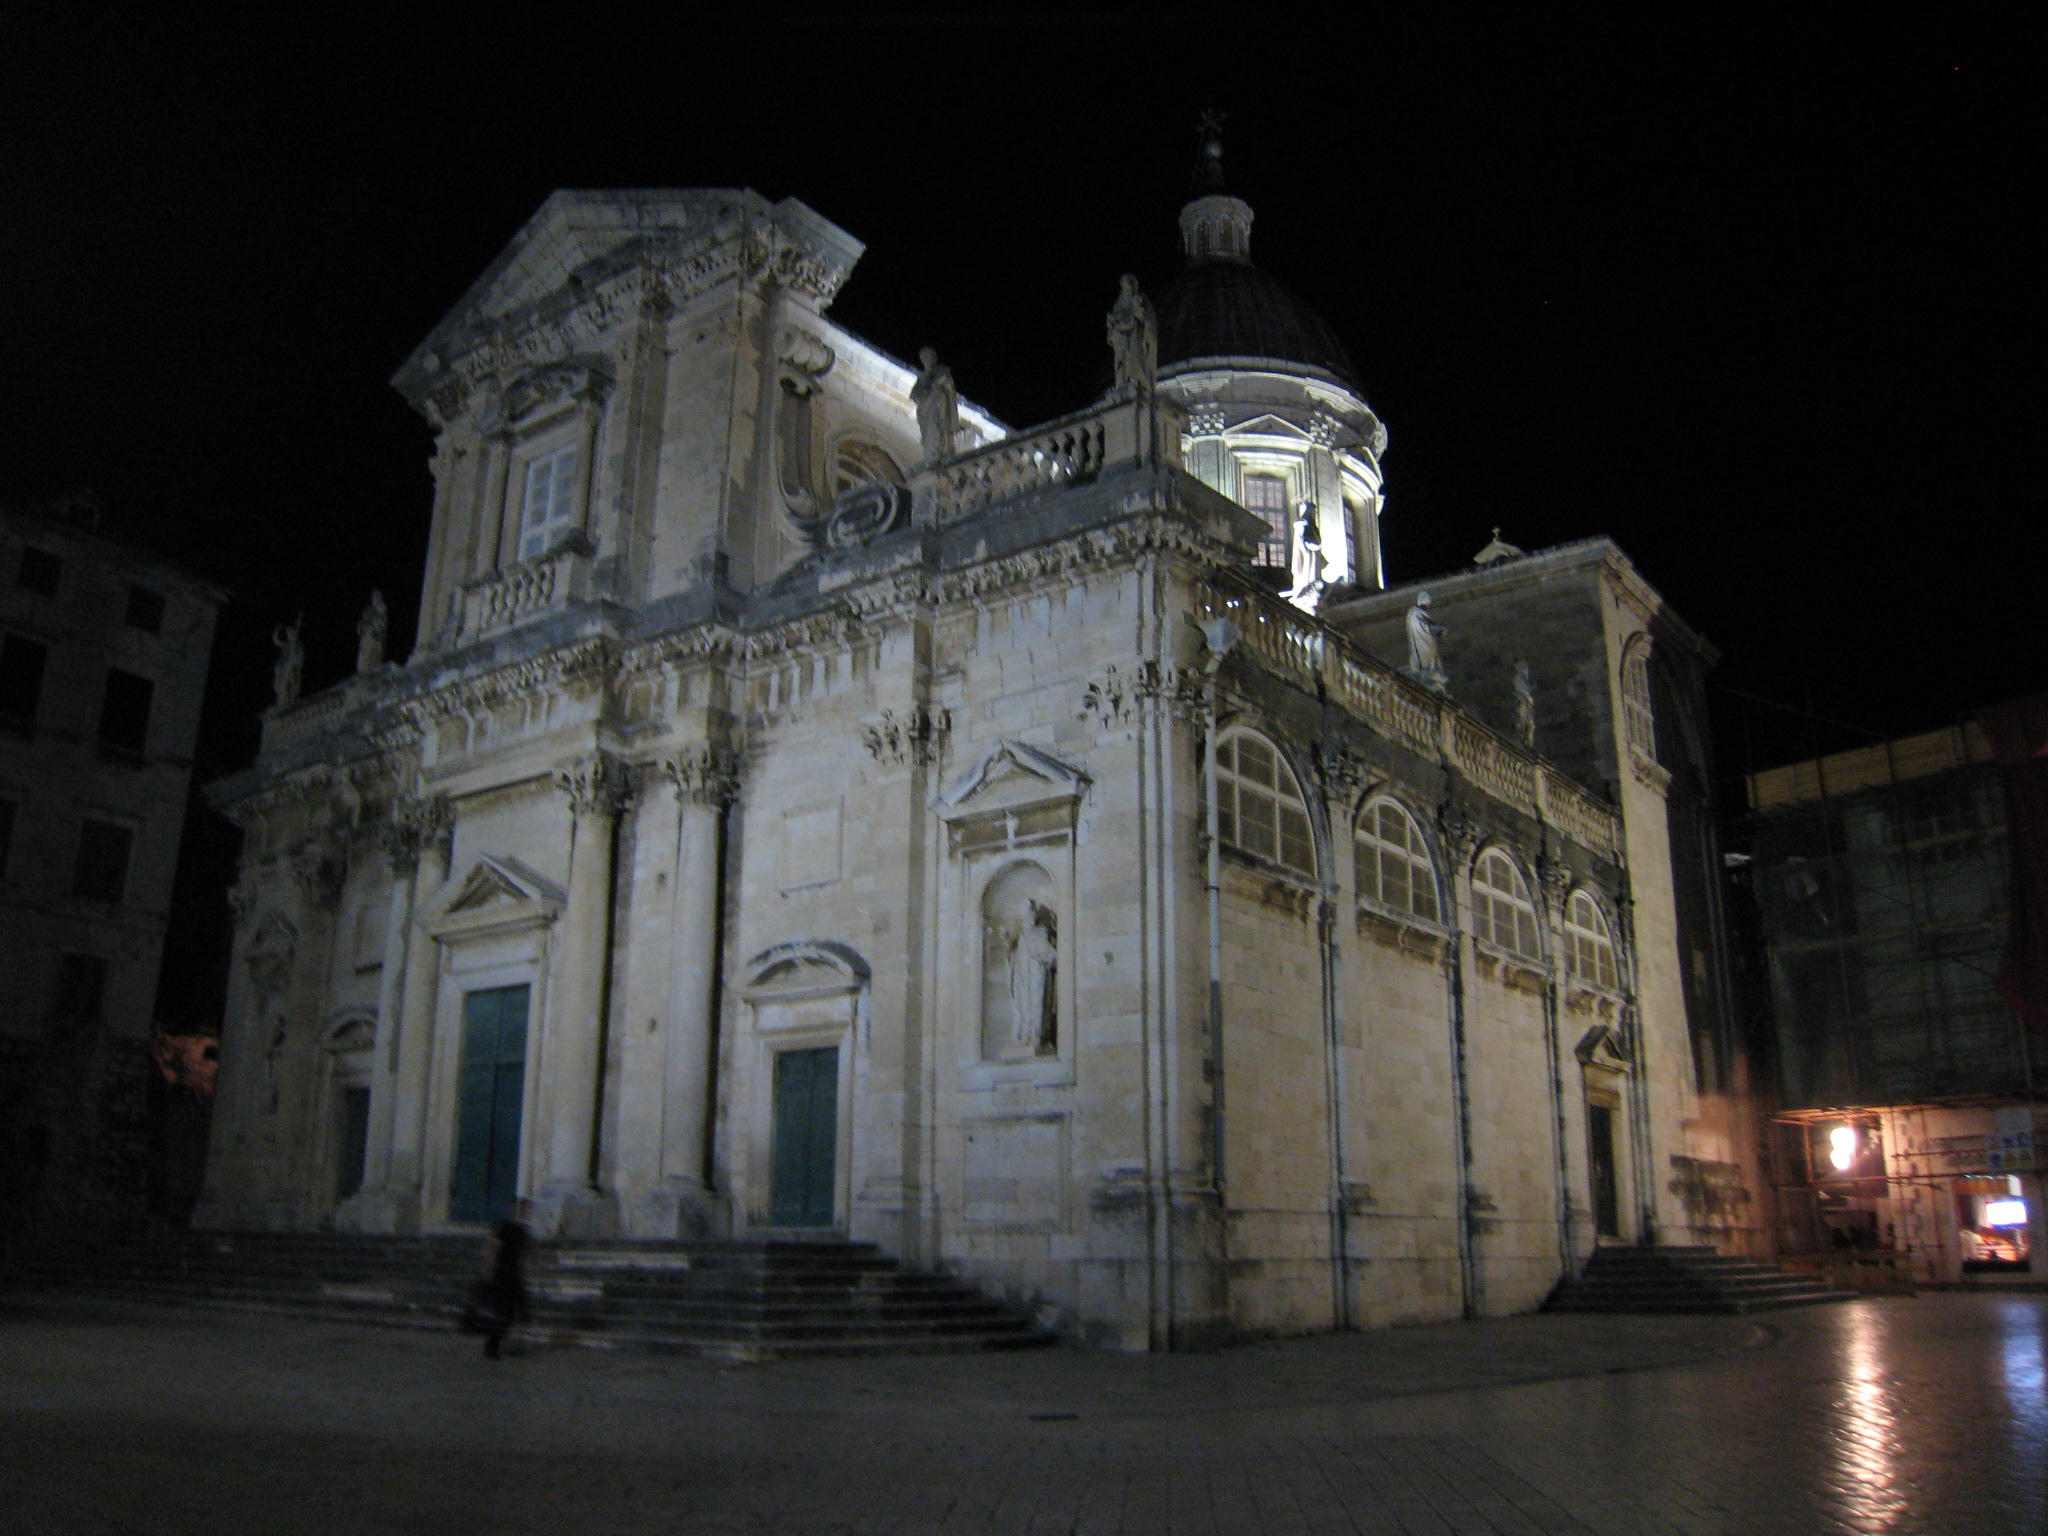
\includegraphics[width=\linewidth]{images/intro_fig/dubrovnik_night_query.jpg}
		\end{minipage}
		\hfill $\rightarrow$ 	\hfill
		\begin{minipage}{0.3\linewidth}
			\centering
			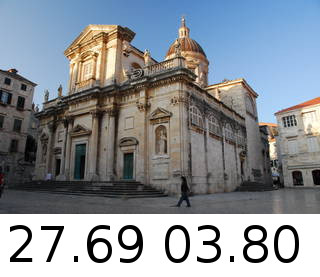
\includegraphics[width=0.8\textwidth]{images/intro_fig/dataset/8.jpg}
		\end{minipage}
	    \hfill $\rightarrow$ 	\hfill
		\begin{minipage}{0.3\linewidth}
			\centering
			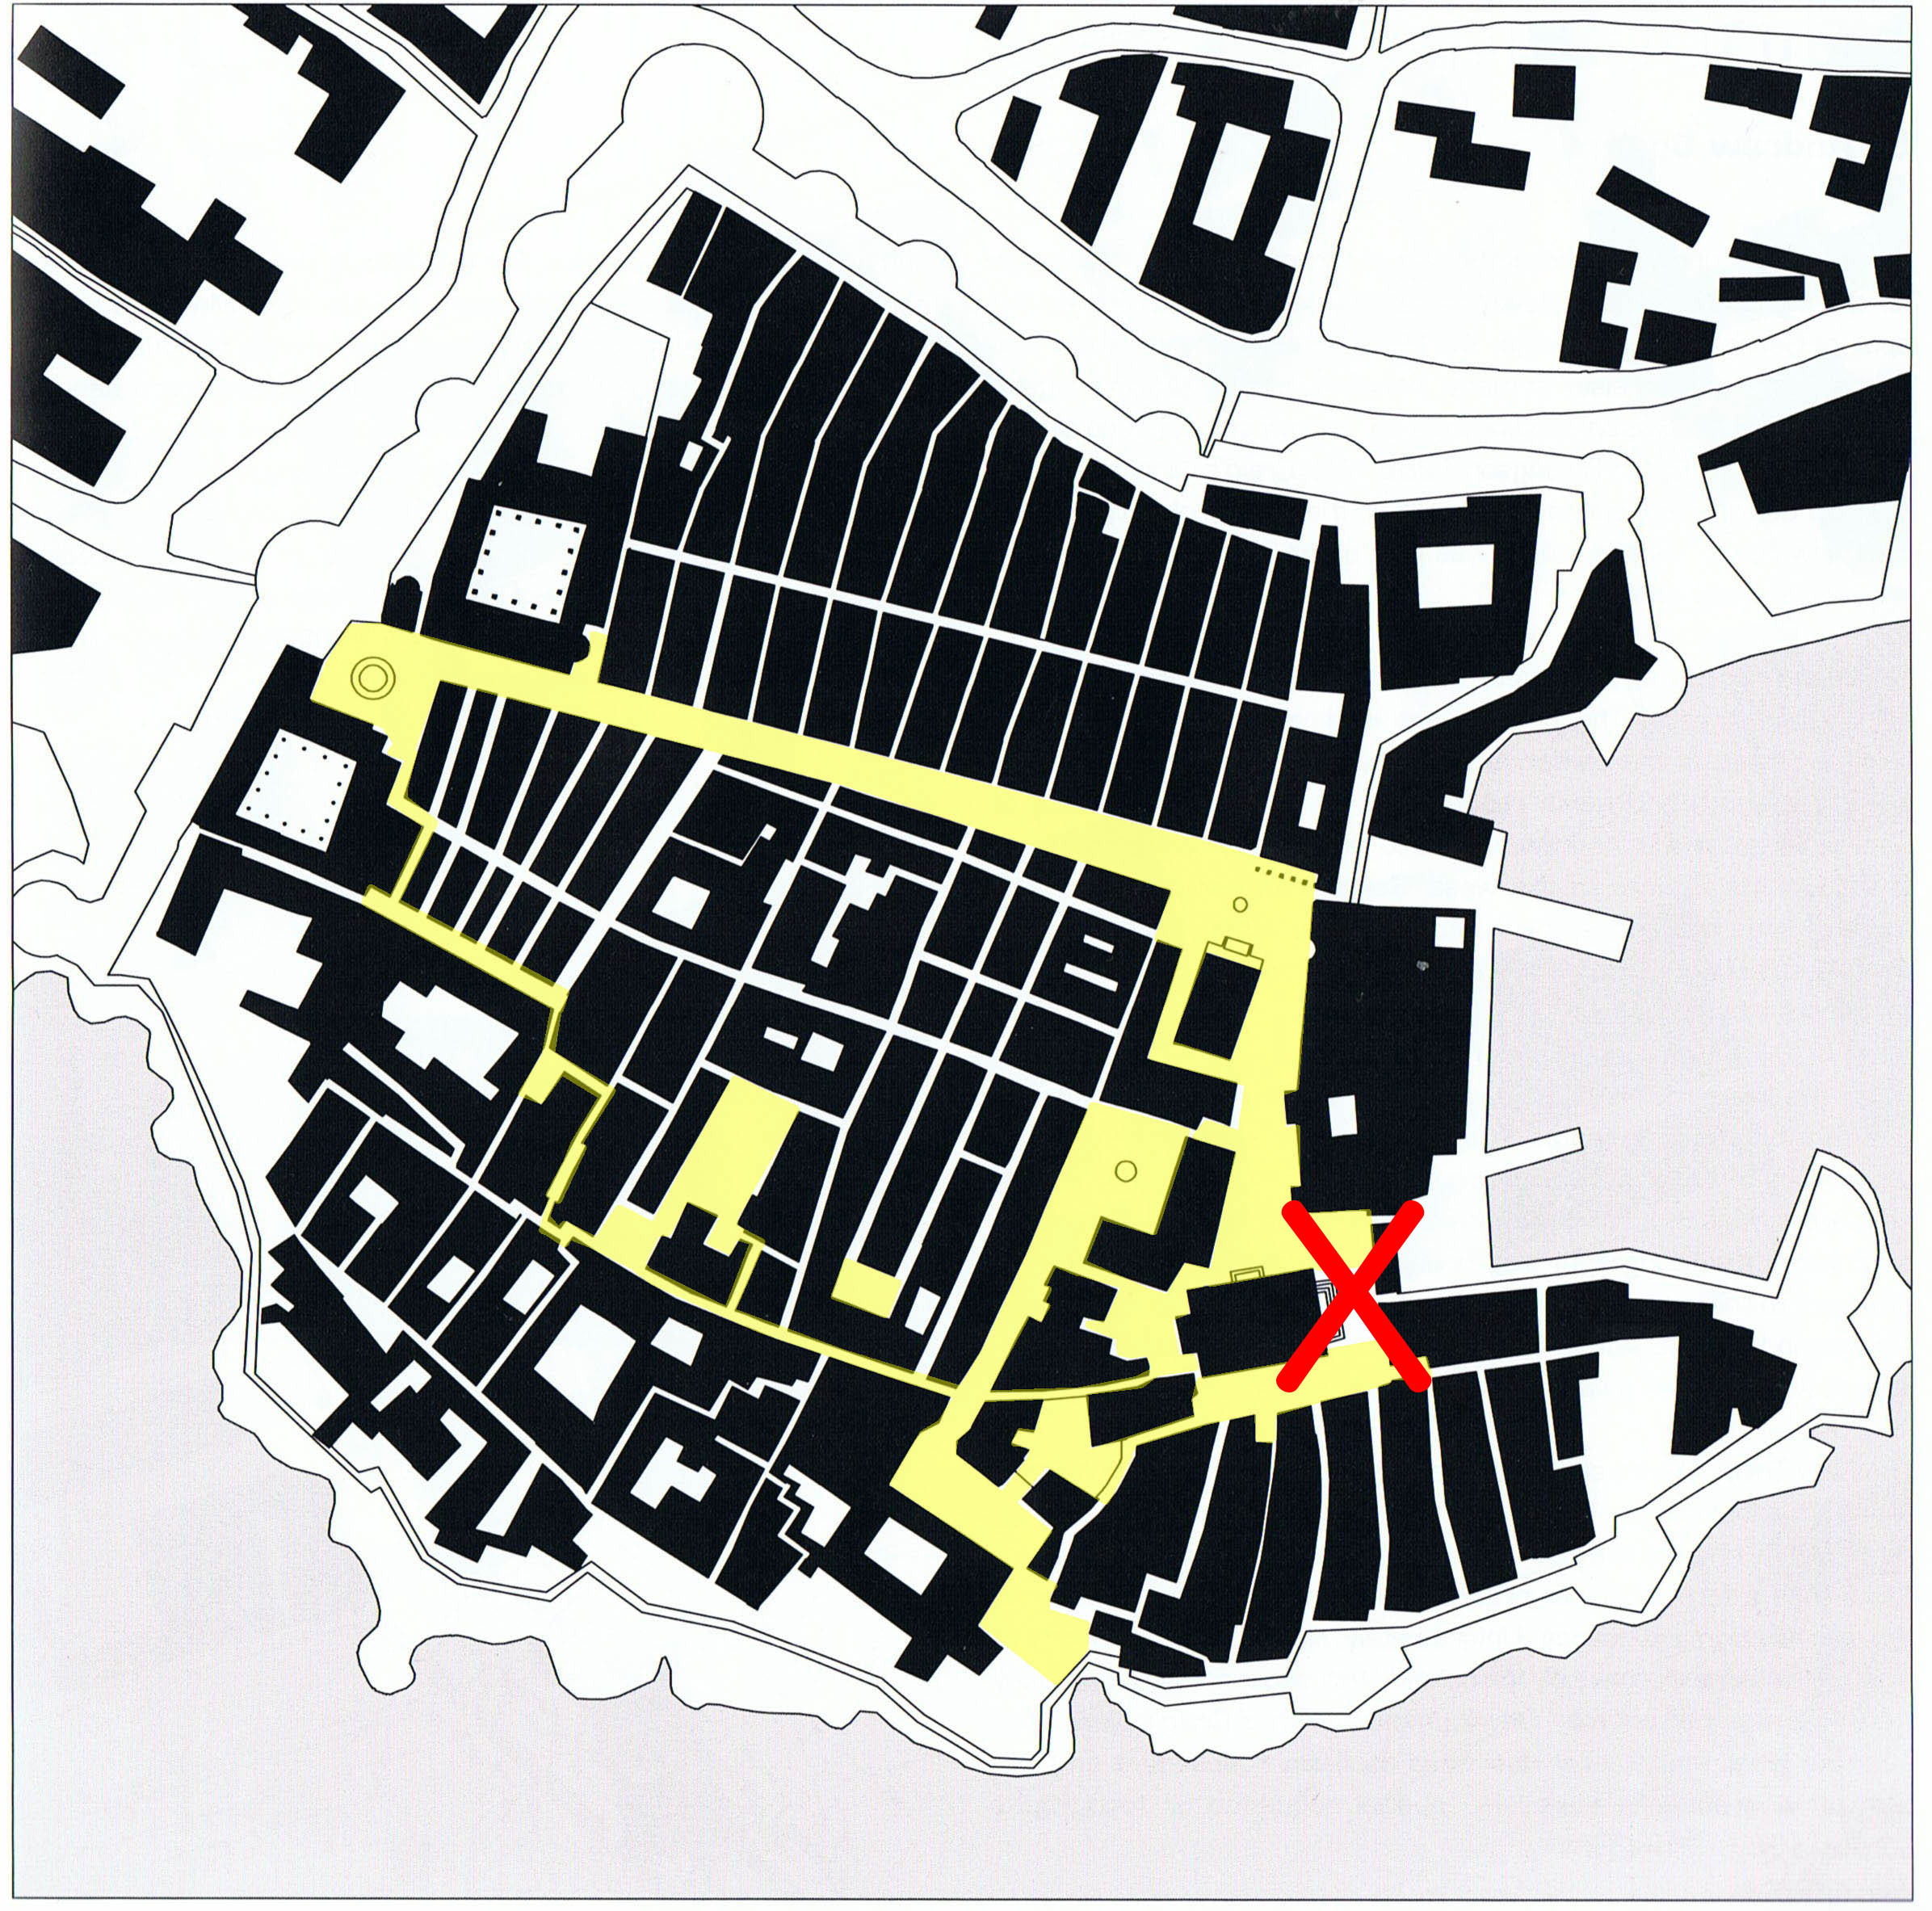
\includegraphics[width=\linewidth]{images/intro_fig/dubrovnik_map_marked.jpg}
		\end{minipage}
	}
\end{frame}


\begin{frame}{Indirect methods: Pipeline}
	
	We propose a new data representation for solving indirect VBL.
	\vfill	
	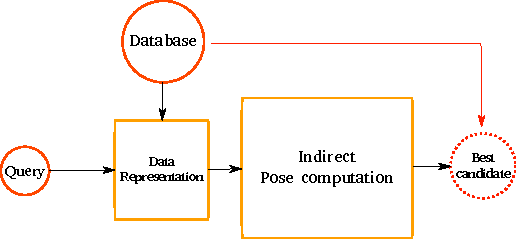
\includegraphics{vect/keys_comp_indirect.pdf}
	
\end{frame}

\begin{frame}{Various modalities}
	In this work, we tackle the problem of VBL with \textbf{not only} images.
	\vfill
	\begin{minipage}{0.55\linewidth}
		\begin{block}{Modalities that could be used}
			\begin{itemize}
				\item<1-> \textbf{Image} (main modality)
				\item<2-> Depth map
				\item<3-> Reflectance
				\item<4> Semantic information
				\item<4> ...
			\end{itemize}
		\end{block}
	\end{minipage}
	\hfill
	\begin{minipage}{0.4\linewidth}
		\centering
		\only<1>{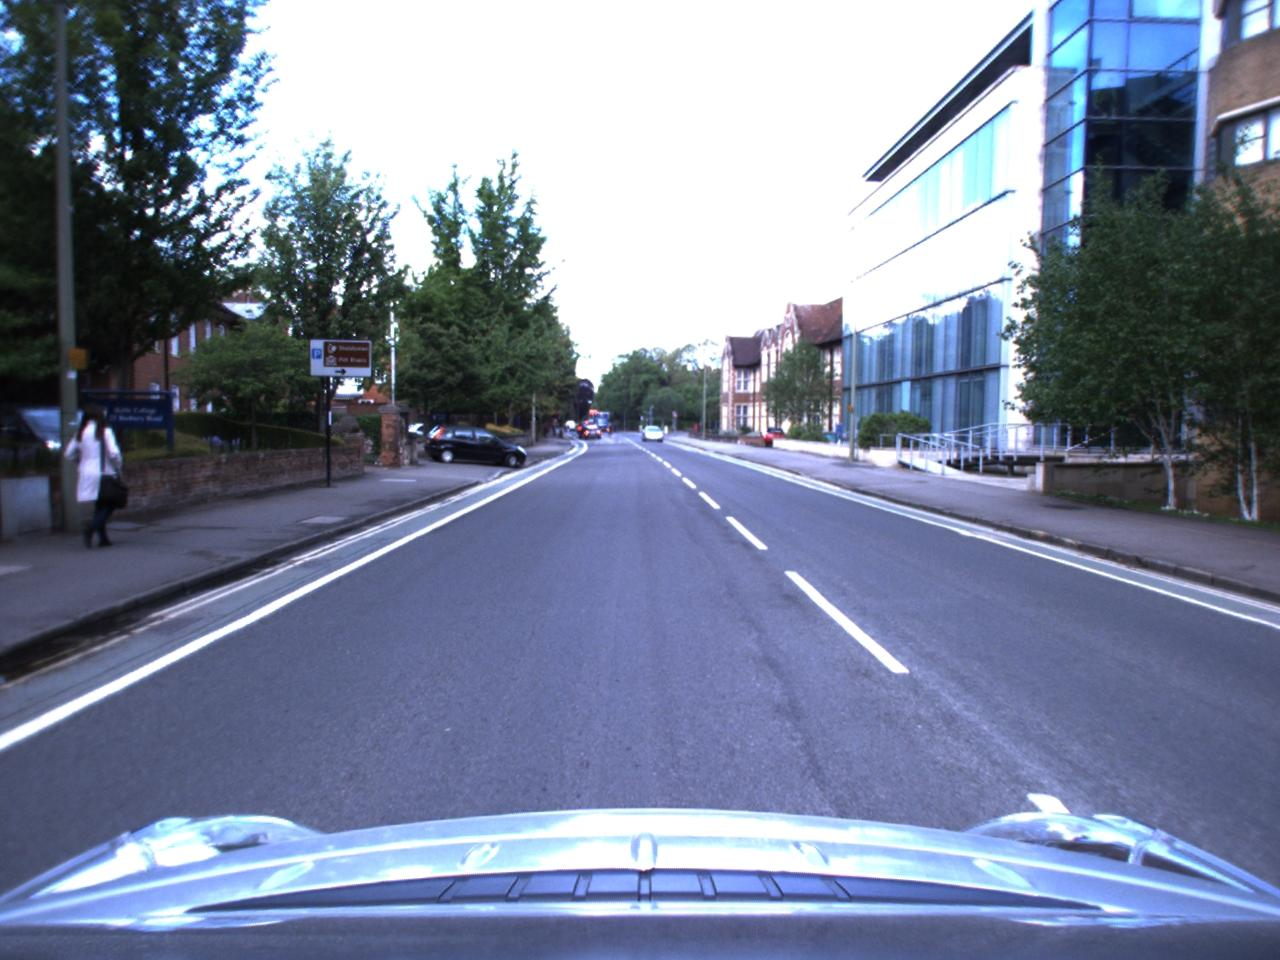
\includegraphics[width=\linewidth]{intro_fig/modalities/rgb}}
		\only<2>{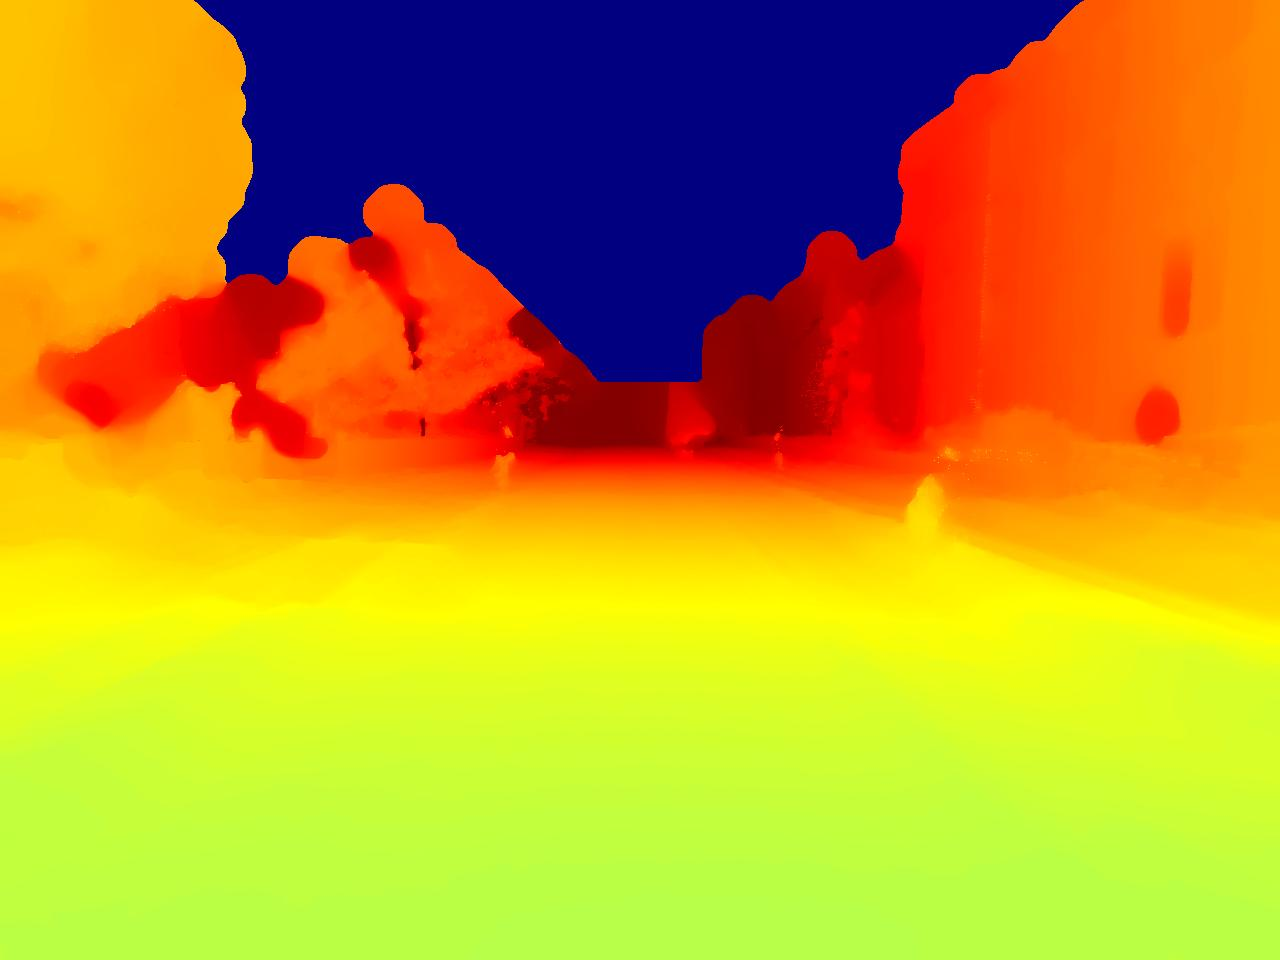
\includegraphics[width=\linewidth]{intro_fig/modalities/depth}}
		\only<3>{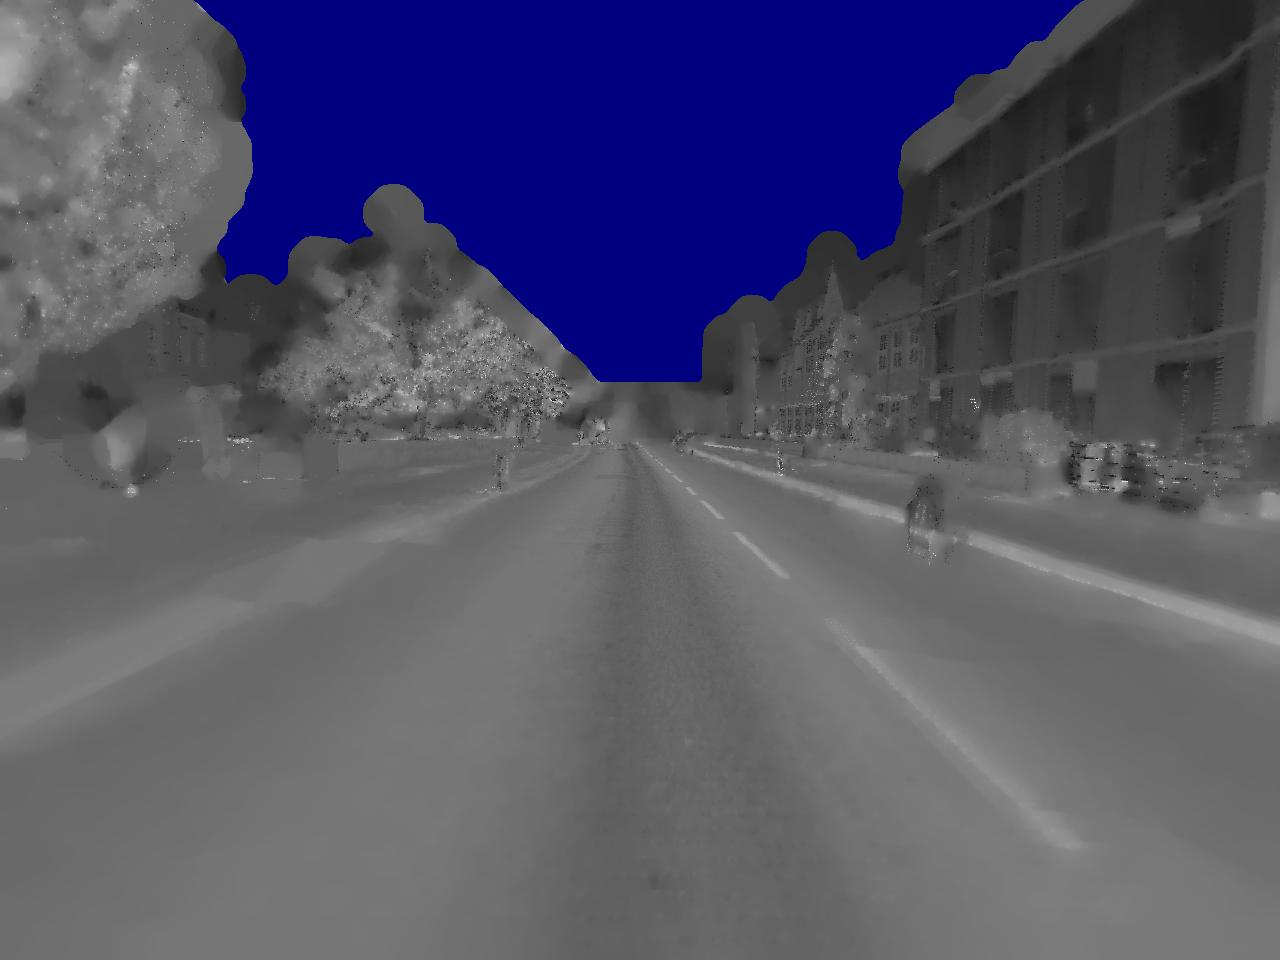
\includegraphics[width=\linewidth]{intro_fig/modalities/ref}}
		\only<4>{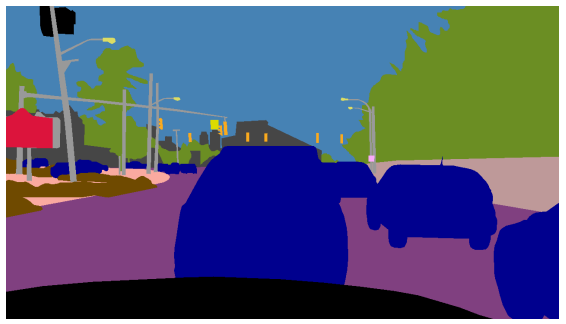
\includegraphics[width=\linewidth]{intro_fig/modalities/semantic}}
	\end{minipage}
\end{frame}

\begin{frame}{Heterogeneous modalities}
	\vfill
	\begin{block}{Available data}
		\centering
		\begin{tabular}{c | c}
			\textbf{Training data type} & \textbf{Testing data type} \\
			\hline
			\textbf<1>{RGB + Depth} & \textbf<2>{RGB}  \\
		\end{tabular}
	\end{block}
	\vfill
	\begin{figure}[t]
		\centering
		\uncover<1->{
		\begin{minipage}[b]{0.65\linewidth}
			\centering
			{\footnotesize \textbf{Multi-modal} training dataset}	
	
			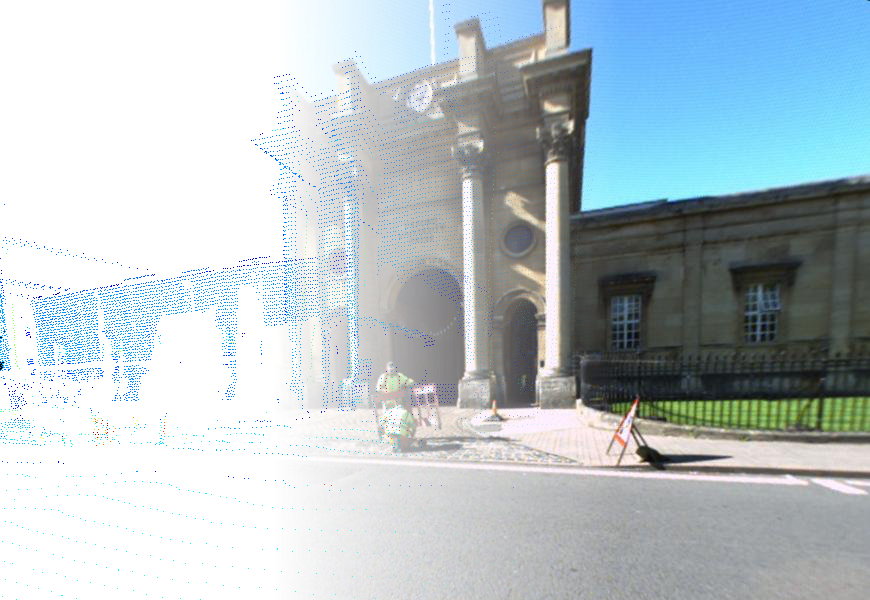
\includegraphics[width=0.51\linewidth]{images/intro_fig/mod0.png}\hspace{0.05mm}
			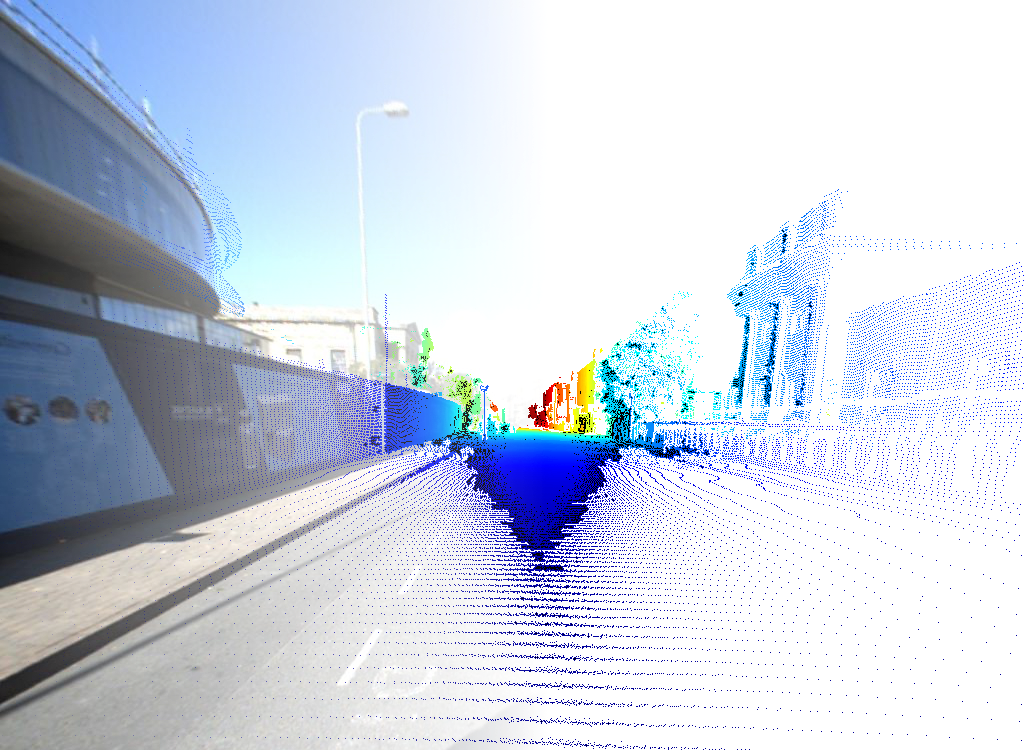
\includegraphics[width=0.47\linewidth]{images/intro_fig/mod1.png}
		\end{minipage}
		}
		\uncover<2>{
		\begin{minipage}[b]{0.32\linewidth}
			\centering
			{\footnotesize \textbf{Single modality} data at test time}
	
			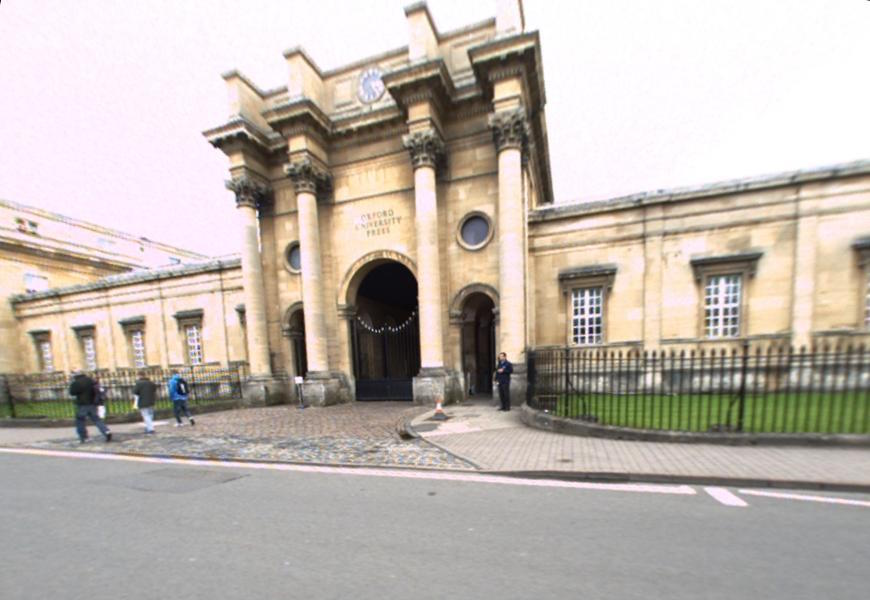
\includegraphics[width=0.85\linewidth]{images/intro_fig/q.jpg}
		\end{minipage}
		}
	\end{figure}
\end{frame}
